\subsection{Формула Кельвина-Стокса}
\begin{theorem}[Кельвин, Стокс]
    Пусть $S = \overline{r}(\overline{G})$~---~поверхность. Пусть выполнены следующие условия: 
    \begin{itemize}
        \item $S$~---~простая гладкая поверхность в $\R^3$; $G \subset \R^2_{uv}$
        \item $\overline{r} \in C^2(\overline{G}, \R^3)$
        \item $\partial G$~---~простой кусочно-гладкий контур
        \item $S$~---~ориентируема и $\partial S^+$~---~положительно ориентирована относительно $S$.
        \item $\exists \Omega: \R^3 \supset \Omega \supset S$, $\Omega$~---~открытое и пусть $\overline{a} \in C^1(\Omega, \R^3)$
    \end{itemize}
    Тогда \[\iint\limits_{S} (\rot \overline{a}, \overline{ds}) = \int\limits_{\partial S^+} (\overline{a}, \overline{dr})\]
\end{theorem}
\begin{proof}
    \textbf{Шаг 1.} Пусть \[\overline{a} = \begin{pmatrix}
        P \\ Q \\ R
    \end{pmatrix}\]
    Поскольку ротор линеен, мы можем доказать теорему только для \[\overline{a}_1 = \begin{pmatrix}
        P(x, y, z) \\ 0 \\ 0
    \end{pmatrix}, \text{ помня что } \begin{pmatrix}
        x \\y \\x
    \end{pmatrix} = \begin{pmatrix}
        x(u(t), v(t)\\ y(u(t), v(t))\\ z((u(t), v(t)) \\
    \end{pmatrix}\]
    И показать \[\iint\limits_S (\rot \overline{a}_1, \overline{ds}) = \int\limits_{\partial S^+} (\overline{a}_1, \overline{dr})\]
    \textbf{Шаг 2.} Поскольку $S$~---~простая гладкая поверхность, то у неё есть две ориентации: \[ \overline{n} = \pm \dfrac{\overline{r}'_u \times \overline{r}'_v}{|\overline{r}'_u \times \overline{r}'_v|}\]
    Докажем для положительной ориентации, для другой доказательство аналогично. Рассмотрим ситуацию, где $(u, v)$~---~правая СК, и $\partial G^+$~---~ориентирована положительно относительно $G$. Тогда \[\int\limits_{\partial S^+} (\overline{a}_1, \overline{dr}) = \int\limits_{\partial S^+} Pdx = \int\limits_\alpha^\beta Px'_tdt = \int\limits_\alpha^\beta P(x'_uu'_t + x'_vv'_t)dt = \int\limits_{\partial G^+} Px'_udu + Px'_vdv = (*)\]
    \textbf{Шаг 3.} Теперь используем формулу Грина: \[(*) = \iint\limits_G \left[(Px'_v)'_u - (Px'_u)'_v \right] dudv = \iint\limits_G (P'_ux'_v + Px''_{vu} - P'_vx'_u - Px''_{uv})dudv = \iint\limits_G (P'_ux'_v - P'_vx'_ududv) = (*)\]
    Именно здесь требуется условие $\overline{r} \in C^2(\overline{G}, \R^3)$. У нас сокращаются компоненты $Px''_{uv} = P''_{vu}$. \\
    \textbf{Шаг 4.}Поскольку: \begin{equation*}
        \begin{cases}
            P'_u = P'_xx'_u + P'_yy'_u + P'_zz'_u \\
            P'_v = P'_xx'_v + P'_yy'_z + P'_zz'_v
        \end{cases}
    \end{equation*}
    То \[(*) = \iint\limits_G P'_y(y'_ux'_v - y'_vx'_u) + P'_z(z'_ux'_v - z'vx'_u)dudv = \iint\limits_G P'_z\dfrac{\partial(z, x)}{\partial(u, v)} - P'_y \dfrac{\partial(x, y)}{\partial(u, v)}\]
    \textbf{Шаг 5.} С другой стороны, поскольку \[\rot \overline{a}_1 = \begin{vmatrix}
        i & j & k \\ \dfrac{\partial}{\partial x} & \dfrac{\partial}{\partial y} & \dfrac{\partial}{\partial z} \\ P & 0 & 0
    \end{vmatrix} = \begin{pmatrix}
        0 \\ P'_z \\ -P'_y
    \end{pmatrix}\]
    То \[\iint\limits_S (\rot \overline{a}_1, \overline{ds}) = \iint\limits_G \begin{vmatrix}
        0 & P'_z & -P'_y \\ x'_u & y'_u & z'_u \\ x'_v & y'_v & z'_v
    \end{vmatrix} dudv = \iint\limits_G P'_z \dfrac{\partial(z, x)}{\partial(u, v)} - P'_y \dfrac{\partial(x, y)}{\partial(u, v)}dudv\]
    Но это в точности то что нам нужно, и таким образом получается что теорема доказана.
\end{proof}
\begin{note}
    Теорема Кельвина-Стокса справедлива при более слабом условии: $\overline{r} \in C^1(\overline{G}, \R^3)$.
\end{note}
\begin{theorem}[Кельвин-Стокс для кусочной-гладкой поверхности]
    Пусть $S \in \R^3$~---~кусочно-гладкая поверхность. Пусть $\partial S^+$~---~ориентированный положительно относительно $S$ край, состоящий из конечного числа простых кусочно-гладких кривых. Пусть задано открытое $\Omega \supset S$ и в нём $\overline{a} \in C^1(\Omega, \R^3)$. Тогда \[\iint\limits_S (\rot \overline{a}, \overline{ds}) = \int\limits_{\partial S^+} (\overline{a}, \overline{dr})\]
\end{theorem}
\begin{proof}
    Используя замечание и предыдущую теорему для каждого куска мы получаем формулу Стокса. Далее, суммируя по всем кускам мы получим необходимое. Ключевой момент~---~при суммировании циркуляций для соседних кусков циркуляция по общему краю равна 0, в силу противоположных ориентаций.
\end{proof}

\section{Элементы теории поля}
\subsection{Геометрическое определение ротации}
\noindent 
    \begin{minipage}{0.75\textwidth}
   \begin{theorem}
    Пусть в непустой области $\Omega \subset R^3$ задано гладкое поле $\overline{a} \in C^1 (\Omega, \R^3)$. Тогда $\forall \overline{r}_0 \in \Omega$ справедливо следующее равенство: \[ (\overline{n}, \rot \overline{a}(\overline{r}_0)) = \lim\limits_{\delta \rightarrow +0} \dfrac{1}{\pi \delta^2} \int\limits_{\partial S^+_\delta(\overline{r}_0)} (\overline{a}, \overline{dr}).\]
    Где $\overline{n}$~---~вектор, задающий положительную ориентацию, $S^+_\delta$~---~окружность радиуса $\delta > 0$ лежащая в плоскости, проходящая через $\overline{r}_0$ перпендикулярно вектору $\overline{n}$. Ориентация $\partial S^+_\delta(\overline{r}_0)$ согласована с $\overline{n}$.
\end{theorem}
       
    \end{minipage}
    \begin{minipage}{0.25\textwidth}
    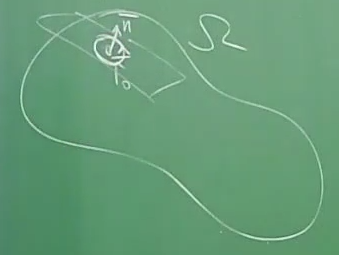
\includegraphics[width=\textwidth]{images/rotor777.png}
    \end{minipage}


\begin{proof}
    Зафиксируем произвольную точку $\overline{r}_0 \in \Omega$.\\
    Так как $\Omega$ открыто, $\exists \delta_0 > 0$: $B_{\delta_0}(\overline{r}_0) \subset \Omega$. $\forall \delta \in (0, \delta_0)$ рассмотрим сечение шара $B_\delta(\overline{r}_0)$ плоскостью, проходящей через $\overline{r}_0$ перпендикулярно $\overline{n}$. Применим теорему Стокса к получившемуся кругу и получим: \[\dfrac{1}{\pi \delta^2} \int\limits_{\partial S^+_\delta}(\overline{a}, \overline{dr}) = \dfrac{1}{\pi \delta^2} \iint\limits_{S^+_\delta} (\rot \overline{a}, \overline{ds})\] 
    Рассмотрим \[\biggr| (\overline{n}, \rot \overline{a})(\overline{r}_0) - \dfrac{1}{\pi \delta^2} \iint\limits_{S^+_\delta} (\rot \overline{a}, \overline{n})ds \biggr| = (*)\]
    Покажем что $(*)$ стремится к 0, при $\delta \rightarrow +0$: \[\dfrac{1}{\pi \delta^2}\biggr| \iint\limits_{S^+_\delta} (\overline{n}, \rot \overline{a}(\overline{r}_0)) - (\overline{n}, \rot \overline{a}(\overline{r}))\biggr|ds \leq \dfrac{1}{\pi \delta^2} \iint\limits_{S^+_\delta} \bigr| (\overline{n}, \rot \overline{a}(\overline{r}) - \rot \overline{a}(\overline{r}_0))\bigr|ds \leq \] \[\leq \dfrac{1}{\pi \delta^2} \iint\limits_{S^+_\delta} \biggr|\Big(\overline{n}, \ \sup\limits_{S^+_\delta}|\rot \overline{a}(\overline{r}) - \rot \overline{a}(\overline{r}_0)|\Big)\biggr|ds = \biggr| \Big(\overline{n}, \sup\limits_{S^+_\delta}|\rot \overline{a}(\overline{r}) - \rot \overline{a}(\overline{r}_0) \Big)|\biggr| \xrightarrow{\delta \rightarrow +0} 0\]
    В силу непрерывности ротора, как функции от $r $
\end{proof}
\subsection{Потенциальные поля}
\begin{definition}
    Пусть $\Omega$~---~непустая область в $\R^n$ и $\overline{a} \in C(\Omega, \R^n)$. Будем говорить что $\overline{a}$~---~потенциально в $\Omega$, если существует $\phi \in C^1(\Omega, \R)$ т.ч. $\overline{a} = \grad \phi$; $\phi$ будем называть потенциалом.
\end{definition}
\begin{theorem}
    Пусть $\Omega \subset \R^n$~---~непустая область, $\overline{a} \in C(\Omega, \R^n)$. Следующие условия эквивалентны: 
    \begin{itemize}
        \item Для всякого простого кусочно-гладкого контура $\Gamma \subset \Omega$ выполнено \[\oint\limits_\Gamma (\overline{a}, \overline{dr}) = 0\]
        \item Для любых кусочно-гладких кривых $\Gamma_1$ и $\Gamma_2$ с общим началом и концом и больше нигде не пересекающихся справедливо \[\int\limits_{\Gamma_1} (\overline{a}, \overline{dr}) = \int\limits_{\Gamma_2} (\overline{a}, \overline{dr})\]
        \item $\overline{a}$ потенциально в $\Omega$
    \end{itemize}
\end{theorem}
\begin{proof}
    Импликация $1) \Rightarrow 2)$ очевидна: пусть у нас есть такие $\Gamma_1$ и $\Gamma_2$. Тогда, если мы применим $1)$ к замкнутому контуру $\Gamma = \Gamma_1^+ \cup \Gamma_2^-$, то мы получим нужное. \\
    Докажем $3) \Rightarrow 1)$. Пусть $\exists \phi: \overline{a} = \grad \phi$. Пусть $\Gamma = \{\overline{r}(t) | t \in [a, b]\}$ и $r(a) = r(b)$~---~кусочно-гладкий контур. Тогда \[\int\limits_\Gamma (\overline{a}, \overline{dr}) = \int\limits_\Gamma (\nabla \phi, \overline{dr}) = \int\limits_a^b (\nabla \phi, \dot{\overline{r}}(t)) dt = (*)\]
    Заметим, что для $\phi \circ \overline{r}$ верно следующее: \[\dfrac{d}{dt}\phi \circ \overline{r}(t) = \phi'_xx'_t + \phi'_yy'_t + \phi'_zz'_t = (\nabla \phi, \dot{\overline{r}}(t))\]
    Т.е. для $(*)$ используя это и формулу Ньютона-Лейбница получим, что \[(*) = \int\limits_a^b \dfrac{d}{dt} \phi \circ \overline{r} dt = \phi \circ \overline{r}(b) - \phi \circ \overline{r}(a) = 0\]
    Теперь докажем импликацию $2) \Rightarrow 3)$. Зафиксируем произвольную точку $\overline{r}_0 \in \Omega$. Положим $\phi(\overline{r}) = \int\limits_\Gamma (\overline{a}, \overline{dr})$ где $\Gamma$~---~кусочно-гладкая кривая без самопересечений, соединяющая $\overline{r}_0$ и $\overline{r}$. 
    \begin{note}
        На самом деле, не очевидно что существует такая кусочно-гладкая кривая; но поскольку область -- линейно-связна, то существует непрерывная кривая $\Gamma$, соединяющая всякие две точки. Значит, поскольку $\Gamma$~---~компактна, и $\R^n \setminus \Omega$~---~замкнуто, то $dist(\R^n \setminus \Omega, \Gamma) > 0$ и тогда $\Gamma$ отделима от $\R^n \setminus \Omega$ некоторой <<трубочкой>>. Значит при достаточно мелком разбиении у нас вписана ломаная в эту трубочку, а значит у нас есть кусочно-гладкая кривая, соединяющая две точки.
    \end{note}
    Заметим, что в силу условия $2)$ определение $\phi$ корректно. Теперь покажем что $\phi$~---~действительно потенциал для $\overline{a}$ в $\Omega$. Зафиксируем произвольную точку $\overline{r}_*$. Существует $\delta_0 > 0$ т.ч. $B_\delta(\overline{r}_*) \subset \Omega$.
    Тогда, если $\overline{l}$~---~произвольный единичный вектор, то для $\delta \in (0, \delta_0)$: \[\phi(\overline{r}_* + t \overline{l}) - \phi(\overline{r}_*) = \int\limits_{\Gamma_l} 
    (\overline{a}, \overline{dr}) = \dfrac{1}{t}\int\limits_0^t (\overline{a}(\overline{r}(\xi)), \overline{l})d\xi \rightarrow (\overline{a}(\overline{r}_*), \overline{l}), t \rightarrow +0\]
    Значит $\dfrac{d\phi}{d\overline{l}}(\overline{r}_*) = (\overline{a}(\overline{r}_*), \overline{l})$
    Из этого и гладкости $\phi$ мы получаем нужное утверждение.
\end{proof}
\begin{definition}
    Поле $\overline{a} \in C^1(\Omega, \R^3)$ называется безвихревым в $\Omega$ если $\rot \overline{a} = 0$ в $\Omega$.
\end{definition}
\begin{definition}
    Пусть дана область $\Omega \subset \R^3$. Она называется поверхностно односвязной если для любого простого кусочно-гладкого контура $\Gamma \subset \Omega$ существует кусочно-гладкая поверхность $S \subset \Omega$ такая, что $\partial S = \Gamma$
\end{definition}
\begin{theorem}
    Пусть задано гладкое поле $\overline{a}$ в некоторой области $\Omega$ пространства $\R^3$. Тогда
    \begin{itemize}
        \item Если $\overline{a}$~---~потенциально, то оно безвихревое
        \item Если $\overline{a}$~---~безвихревое и $\Omega$~---~поверхностно-односвязна, то $\overline{a}$~---~потенциально
    \end{itemize}
\end{theorem}
\begin{proof}
    Пусть $\overline{a}$~---~потенциально. Тогда интеграл по любому замкнутому контуру равен 0. Тогда поле -- безвихревое в силу теоремы о геометрическом смысле ротации. \\
    Пусть $\rot \overline{a} = 0$ в $\Omega$. Поскольку $\Omega$ поверхностно односвязная то для всякого замкнутого кусочно-гладкого контура $\Gamma$ существует поверхность $S \subset \Omega$ т.ч. $\partial S = \Gamma$. Значит применяя теорему Стокса-Кельвина мы получаем \[\int\limits_\Gamma (\overline{a}, \overline{dr}) = \int\limits_S (\rot \overline{a}, \overline{ds}) = 0\]
    И по предыдущей теореме поле $\overline{a}$~---~потенциальное.
\end{proof}
\begin{note}
    Если $\Omega$~---~не поверхностно односвязно, то поле может быть безвихревым но не потенциальным. Пусть $\Omega = \R^3 \setminus Oz$ и \[
    \overline{a} = \begin{pmatrix}
        -\dfrac{y}{x^2 + y^2} \\ \dfrac{x}{x^2 + y^2} \\ 0
    \end{pmatrix}
    \]
    Его ротация очевидно равна 0. Но по такому контуру $\Gamma = \{(\cos t, \sin t) \mid t \in [0, 2\pi]\}$
    циркуляция ненулевая.
\end{note}
    